%\documentclass[12pt]{article}
%\usepackage{amsmath,xcolor,todonotes,graphicx,marvosym,dsfont,import,fullpage,textcomp,colortbl,array,pgfplots,lscape}
%\begin{document}
	\section{Results}
	\subsection {OO-NVU 2.0}
	\subsubsection*{Potassium input signal (figure \ref{fig:1IS})}
	At the top the neuronal \gls{K} input signal is shown. This input signal is pumped into the SC by the \gls{NE}. As a result of that, there is more \gls{K} taken up by the \gls{AC} in the beginning of the input pulse, and released at the end of the input pulse. In the second graph the membrane potential of the AC is shown over time. When the \gls{K} concentration in the SC is increased the membrane voltage depolarises and when the \gls{K} concentration in the SC decreases the membrane potential repolarises again.
	In the third graph the fluxes into the PVS are shown. In blue the flux by the astrocytic BK channel, and in green the flux by the KIR channel in the SMC is shown. The drop in the middle of the KIR flux is caused because the SMC becomes in a oscillatory state and therefore the efflux by the KIR channel follows the \gls{Ca} waves inside the SMC.
	The bottom figure shows the \gls{K} concentration in the PVS.
	
	\subsubsection*{Neurovascular Coupling Overview (figure \ref{fig:1})}
	
	\subsubsection*{AC State Variables (figure \ref{fig:2})}
	
	\subsubsection*{AC Fluxes (figure \ref{fig:3})}
	
	\subsubsection*{SMC EC State Variables and Coupling (figure \ref{fig:4})}
	
	\subsubsection*{SMC Fluxes (figure \ref{fig:5})}
	
	\subsubsection*{EC Fluxes (figure \ref{fig:6})}
	
	\subsubsection*{Contraction Model and Radius (figure \ref{fig:7})}
	
	

	\subsubsection*{Solutions of astrocyte and BK-channel equations (figure \ref{fig:7ACe})}
	 The top 4 graphs display the concentrations of \gls{K}, \gls{Ca} \gls{IP3} and EET in the astrocyte. These concentrations, together with the membrane voltage showed in the right bottom graph, all contribute to the opening of the BK-channel in their own way. The open state of the BK channel determines the potassium flux from the astrocyte to the perivascular spcace, where it induces vascular contraction.
	
	\subsubsection*{SMC and EC fluxes (figure \ref{fig:2SMCF} and \ref{fig:3ECF})}
	In these figures the coupling and the fluxes in the SMC and EC are shown. When one of the fluxes is negative, it means that the direction of the flux is in the opposite than it is defined in the equations. These figures show that when the neuronal signal is given, the VOCC closes and that the SMC goes into an oscillatory state. 
	
	\subsubsection*{Conservation equations (figure \ref{fig:4DFDT})}
	The graphs in this figure shows the solutions of the differential equations of the \gls{SMC} and \gls{EC}. The graphs on the left side are the SMC results, and at the right side the EC results. From top to bottom the following parameters are shown over time: the intracellular \gls{Ca} concentration, the \gls{IP3} concentration, the sarcoplasmic (\gls{SMC}) or endoplasmic (\gls{EC}) \gls{Ca} concentration, the membrane voltage and at the bottom for the SMC the open probability of the \gls{K} channels.
	
	\subsubsection*{Hai and Murphy and radius model (figure \ref{fig:5MCm})}
	In this figure the fraction of the four states (M, Mp, AMp, AM) of myosin in the SMC are shown at the top. At the bottom left the fraction of attached cross bridged myosin (the sum of AM and AMp) is shown. And at the bottom right the radius is plotted over time. The increase in vessel diameter is in the expected order of magnitude.
	
	\subsubsection*{Overview from the synaptic cleft to radius change (figure \ref{fig:6NtR})}
	This figure descripes the main pathway from the synaptic cleft to the radius change (leaving out the astrocyte equations which can be found in figure \ref{fig:7ACe}) It starts with a \gls{K} concentration in the synaptic cleft, followed by the flux trough the BK-channel determined in the astrocyte, leading to an increased \gls{K} concentration in the perivascular space. This causes an increased  \gls{K} influx trough the KIR channel, changing the membrane voltage of the SMC. The \gls{Ca} flux through the VOCC increases, decreasing the \gls{Ca} concentration in the SMC and thereby inducing vasodilation. 
		
	
	\begin{landscape}
			
		\begin{figure}[h!]
			\centering
			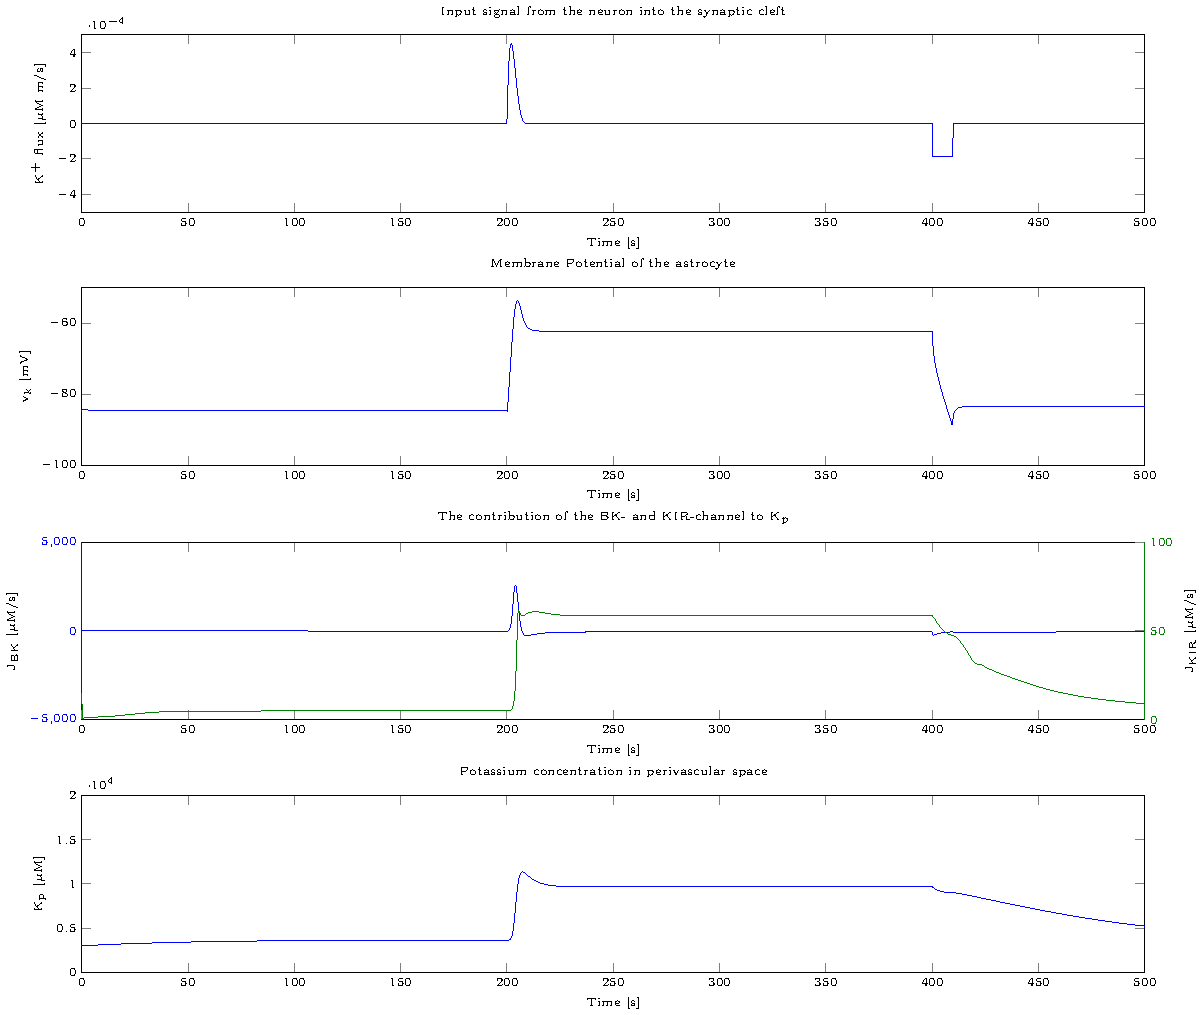
\includegraphics{figures/1_Input_signal.pdf}
			\caption{The input signal.}
			\label{fig:1IS}
		\end{figure}
		
		\begin{figure}[h!]
			\centering
			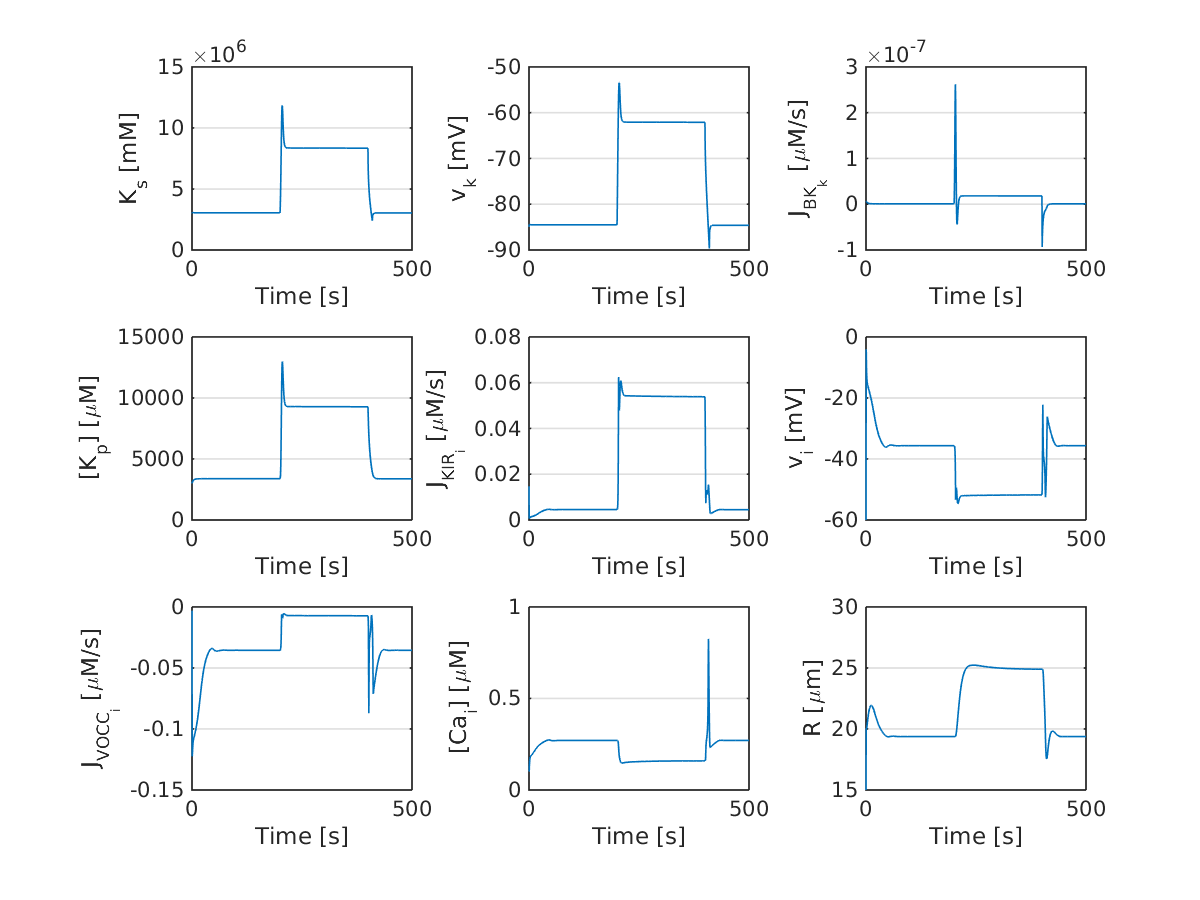
\includegraphics{new_figures/1 Neurovascular Coupling Overview.png}
			\caption{Neurovascular Coupling Overview.}
			\label{fig:1}
		\end{figure}		
		
		\begin{figure}[h!]
			\centering
			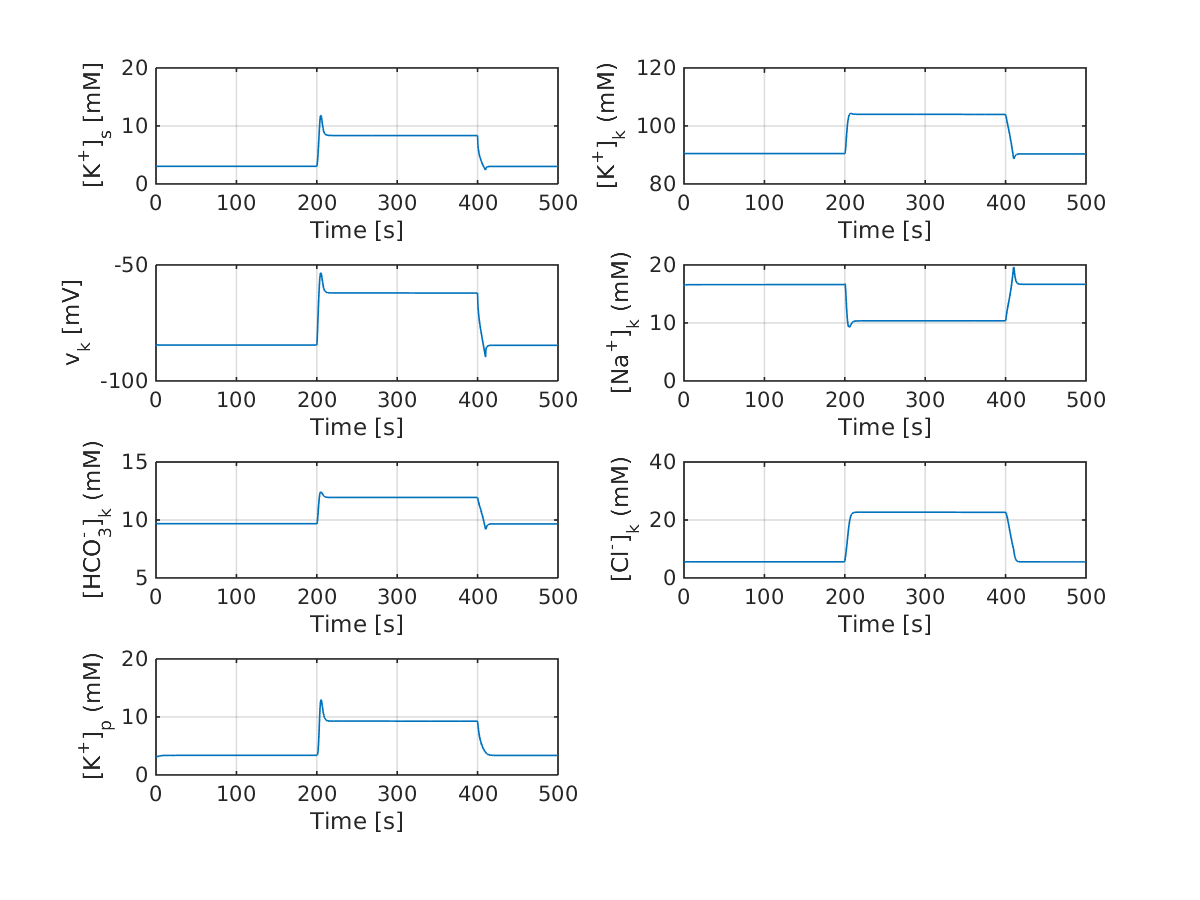
\includegraphics{new_figures/2 AC State Variables.png}
			\caption{AC State Variables.}
			\label{fig:2}
		\end{figure}
	
	
		\begin{figure}[h!]
			\centering
			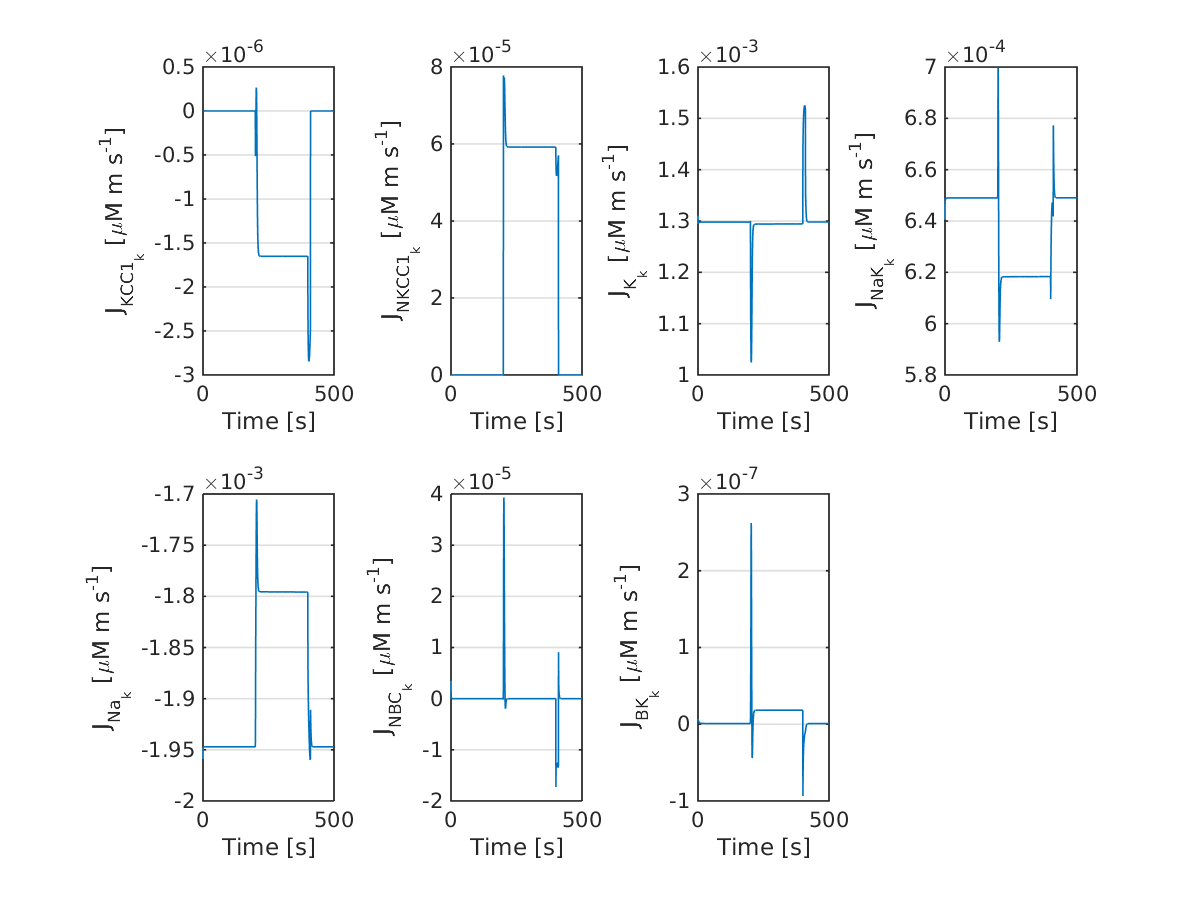
\includegraphics{new_figures/3 AC Fluxes.png}
			\caption{AC Fluxes.}
			\label{fig:3}
		\end{figure}
		
		
		\begin{figure}[h!]
			\centering
			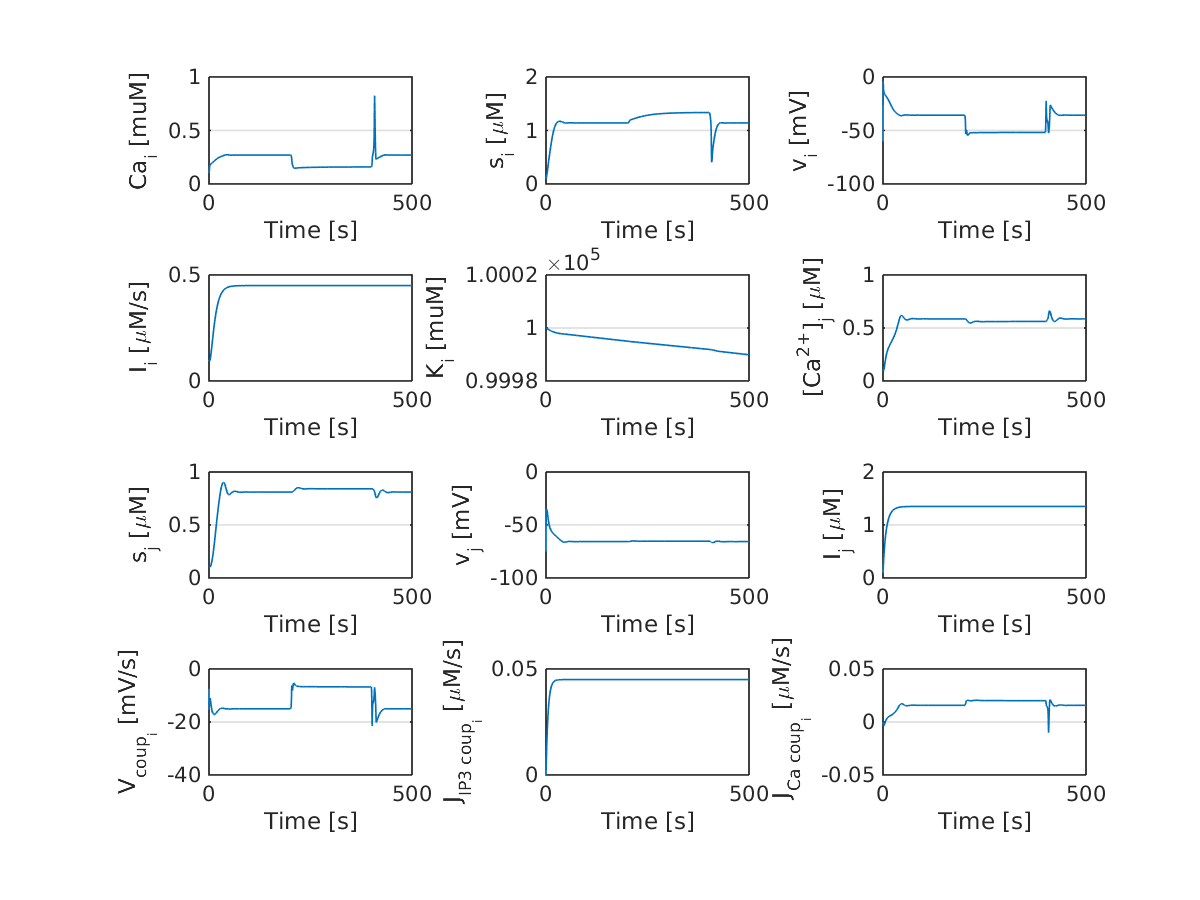
\includegraphics{new_figures/4 SMC EC State Variables and Coupling.png}
			\caption{SMC EC State Variables and Coupling.}
			\label{fig:4}
		\end{figure}
			
		\begin{figure}[h!]
			\centering
			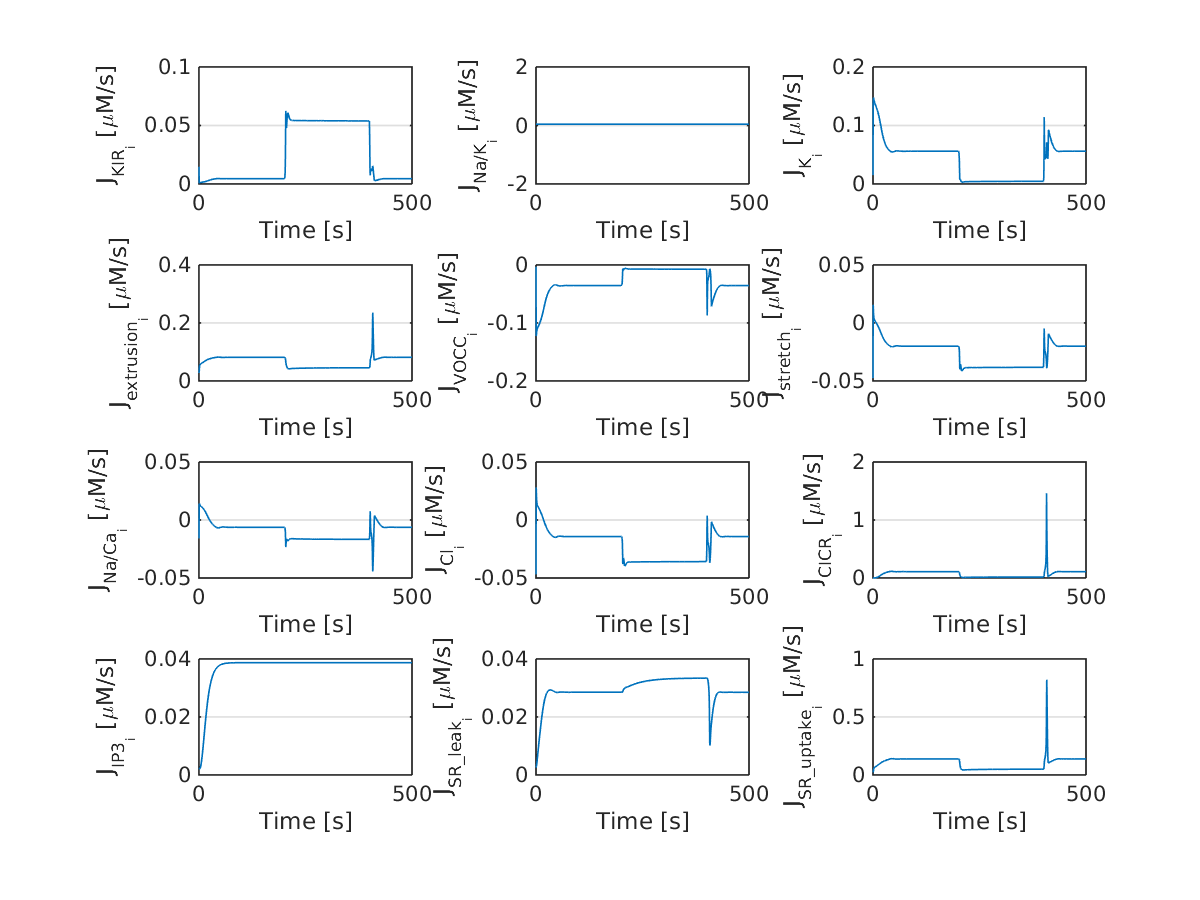
\includegraphics{new_figures/5 SMC Fluxes.png}
			\caption{SMC Fluxes.}
			\label{fig:5}
		\end{figure}
		
		\begin{figure}[h!]
			\centering
			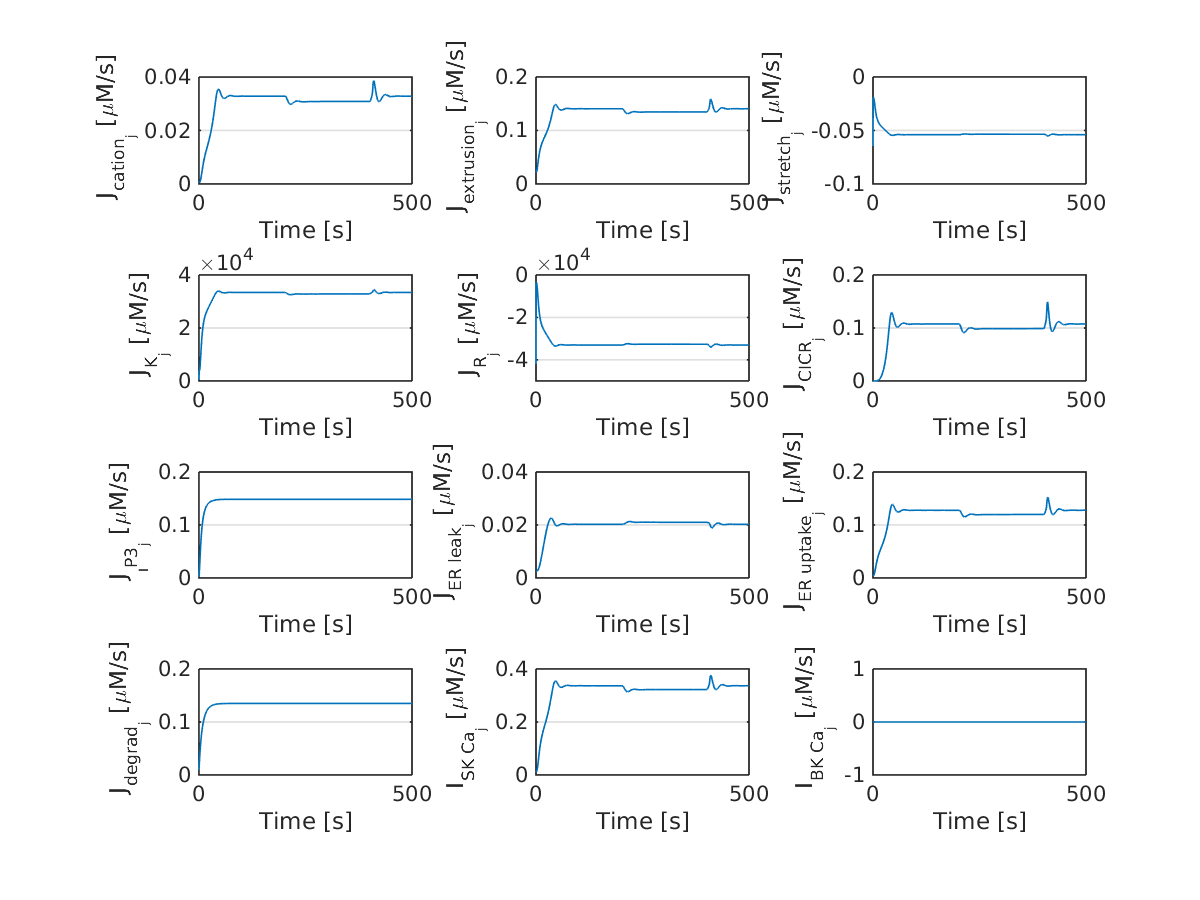
\includegraphics{new_figures/6 EC Fluxes.png}
			\caption{EC Fluxes.}
			\label{fig:6}
		\end{figure}
		
		\begin{figure}[h!]
			\centering
			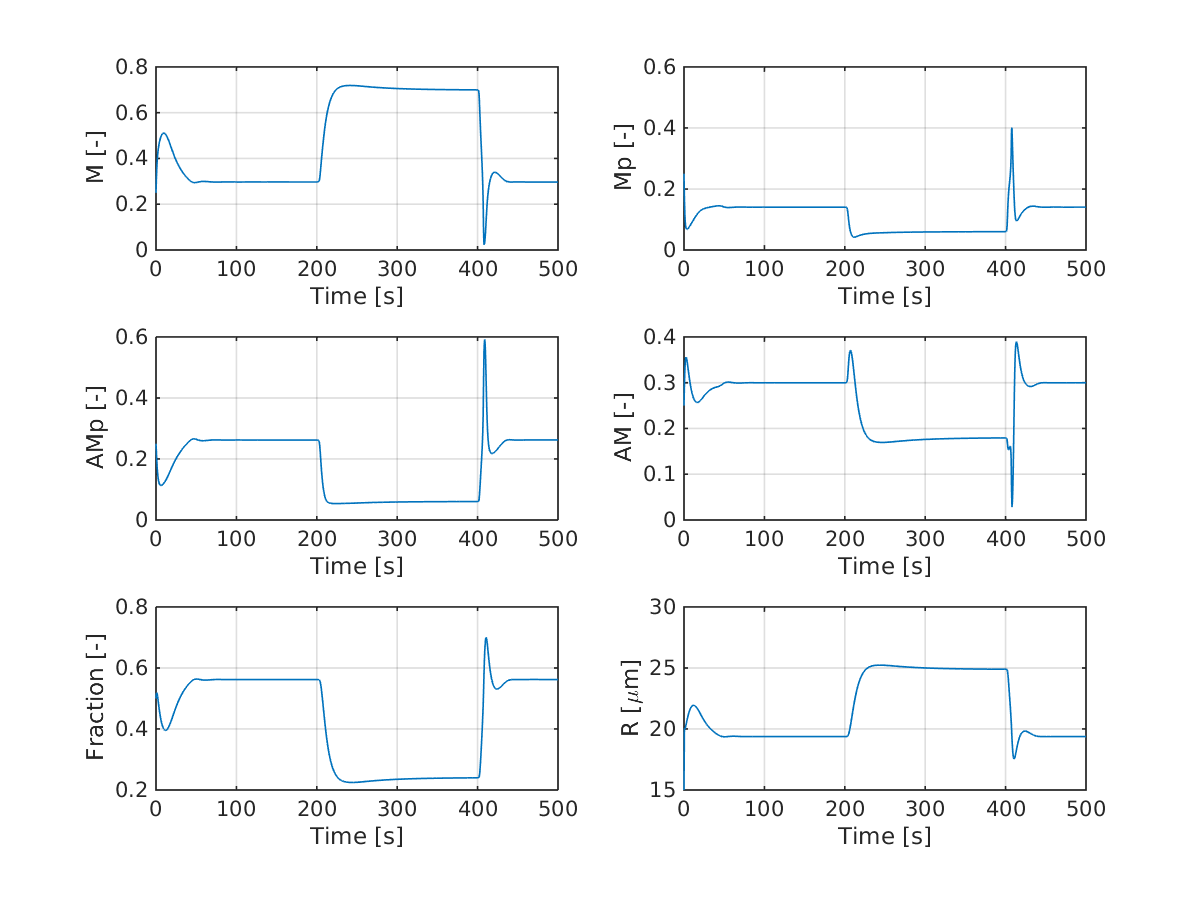
\includegraphics{new_figures/7 Contraction Model and Radius.png}
			\caption{Contraction Model and Radius.}
			\label{fig:7}
		\end{figure}
				
	\end{landscape}
	
